	
\section{Problem \& Motivation}
	Sparse linear algebra is a key component in many scientific simulations
	ranging from quantum physics to fluid and structural mechanics.
	However, iterative numerical methods  
	and important building blocks of sparse linear algebra frequently feature strong 
	data dependencies, making them difficult to parallelize.
	Typically, loop-carried dependencies occur in
	iterative solvers  (e.g., Kaczmarz, Gauss-Seidel) or preconditioners 
	and write conflicts show up in the parallelization of building blocks such 
	as symmetric sparse matrix-vector multiplication.
	Scalable, hardware-efficient parallelization of such methods and kernels is known to be a 
	challenge. \Acrlong{MC} is a widely used approach to enable parallelization
	of iterative solvers with \DK dependency; \eg the 
	red-black Gauss-Seidel algorithm solves the \DONE dependency problem.
	However, most of those standard solutions suffer from low performance
	on modern hardware, are highly problem specific, or require tailored
        sparse matrix storage formats.

	\Acrshort{RACE} addresses these shortcomings by combining ideas from graph traversal
	and \acrlong{MC} to ensure data locality, to generate appropriate levels of parallelism,
	and to enable hardware-efficient parallelization schemes. It is applicable
	to many problems (\ie matrix structures) and general sparse data storage formats.
	
%	In this paper we present a novel approach called \acrshort{RACE} that helps in
%	solving the general distance-k dependency problem for sparse kernels in a
%	hardware efficient manner. The \acrshort{RACE} method is motivated by the
%	shortcomings of multicoloring methods that are frequently used in this scenario.
%	The method works on simple data storage formats
%	like \acrfull{CRS}, and is highly scalable to meet the requirements of 
%	modern CPU based compute nodes. \medskip

\noindent\textbf{Outline}


\noindent	The paper is structured as follows. \Cref{sec:background} describes
	the underlying dependency problems and conventional
	solutions. \Cref{sec:uniqueness} 
	demonstrates the major drawbacks of the existing 
	approaches. We then introduce the \acrshort{RACE} method in \Cref{sec:RACE_method},
	its uniqueness and how its basic design addresses the existing problems. 
	In \Cref{sec:results} we compare \acrshort{RACE} performance for thread-level parallelization of \acrfull{SymmSpMV} to
	available standard solutions including \acrshort{MKL}. Finally we use \acrshort{RACE} to parallelize a sparse eigenvalue solver provided by \acrshort{MKL} and demonstrate  \acrshort{RACE}'s superiority in terms of performance and attainable problem sizes. 
		
	\begin{comment}
	In this paper we present a novel approach called \acrshort{RACE} that helps in
	solving the general \DK dependency problem for sparse kernels in a
	hardware efficient manner. The \acrshort{RACE} method is motivated by the
	shortcomings of multicoloring methods that are frequently used in this scenario.
	The method uses a recursive level-based approach to find optimal permutations
	while preserving good data locality. A thorough performance analysis shows that
	our method achieves high hardware efficiency on modern multi-core architectures
	and it outperforms traditional \acrfull{MC} and \acrshort{MKL} implementations
	by a factor of 2--2.5$\times$. We are on par with \acrfull{ABMC} method for
	small matrices, while for large matrices we gain almost a factor of
	1.5--2$\times$. Owing to the success of parallel implementations of
	sparse kernels having dependencies we further demonstrate first results
	of parallel iterative FEAST eigen solver using CGMN internal solver.
	\end{comment}


\section{Background \& Related Work} \label{sec:background}
%Many numerical methods that come across in sparse linear algebra are hard to 
%parallelize due to dependencies. 
%The two main class of dependencies that occur in this field are \DONE
%dependency as in Gauss-Seidel iteration or a \DTWO dependency as they 
%occur in \acrfull{KACZ} or \acrfull{SymmSpMV}. 
Data dependencies often prevent a straightforward parallelization of sparse linear algebra kernels.
%\setlength{\abovecaptionskip}{20pt}
\begin{algorithm}[b]
	\caption{\label{alg:symmSpMV} \acrshort{SymmSpMV} kernel,  $b=Ax$, in \acrshort{CRS} format.}% Only the upper triangular of the matrix is stored.}
	\begin{algorithmic}[1]
		\Statex{\textcolor{darkgray} {//Loop over all matrix rows}}
		\For{$row=1:nrows$}
			\State{$diag\_idx=rowPtr[row]$}
			\State{$b[row] += A[diag\_idx]*x[row]$}
			\Statex{\hspace{1.5em} \textcolor{darkgray} {//Loop over all non-zero entries in a row}}
			\For{$idx=rowPtr[row]+1:rowPtr[row+1]$} 
				\State{$b[row] += A[idx]*x[col[idx]]$}
				\State{$b[col[idx]] += A[idx]*x[row]$} 
			\EndFor
		\EndFor
	\end{algorithmic}
\end{algorithm}
As a representative and highly relevant example for a \DTWO dependency problem, we use \acrfull{SymmSpMV}. 
\Cref{alg:symmSpMV} shows the pseudo-code of the basic \acrshort{SymmSpMV} kernel 
for upper triangular matrices stored in \acrfull{CRS} \cite{CRS} format. The kernel exploits the symmetry
of the matrix ($A_{ij} = A_{ji}$)  to reduce storage size and overall memory traffic, 
 which is known to be pivotal hardware bottleneck for this operation on all modern compute devices.  
However, \acrshort{SymmSpMV} cannot be parallelized easily as 
different threads working on different rows in parallel could potentially 
write to the same element $b[col[idx]]$,
causing write conflicts.
In terms of graph theory this means a vertex (row in a matrix) and 
its \DTWO neighbors \cite{dist_k_def} cannot be operated on in parallel.
Here we concentrate on such \DTWO dependency problems, although 
the underlying method and library is capable of handling 
the general case of \DK dependencies as well.


A popular approach to solve the above problem is \acrfull{MC}.
The earliest work on coloring is the red-black 
Gauss-Seidel scheme~\cite{RBGS}, which was applied to  matrices with a
 known regular sparsity pattern. 
Later \acrlong{MC} techniques were expanded using graph theory
for general sparse matrices \cite{MC,COLPACK}.
Recent variants like \acrfull{ABMC} \cite{ABMC} tried to improve the performance 
of \acrshort{MC} methods. 
In \cite{feast_mc}, \acrshort{MC} was applied to the Kaczmarz iterative solver \cite{kaczmarz},
 which has the same \DTWO dependency as \acrshort{SymmSpMV}.
Specifically for \acrshort{SymmSpMV} there has been no previous attempt to use 
\acrlong{MC} techniques. General solutions for \acrshort{SymmSpMV} are 
lock-based methods and thread-private target arrays \cite{sparseX,thread_private_symm_spmv}.
Depending on the matrix structure these solutions can lead to performance
 degradation  due to serialization and massive increase in data traffic.
Recent research in this direction uses specialized storage formats like
 CSB \cite{CSB} or RSB \cite{RSB}, but this requires rewriting of existing 
 code and substantial tuning efforts. 

%to Kaczmarz iterative solver having  dependency. 
 
%Many solution to these dependency problems have been proposed, such as 
%locking method and thread-private target arrays \cite{sparseX,thread_private_symm_spmv}.
%But these approaches could lead to performance degradation depending
%on the matrix due to serialization or increase in data traffic respectively.
%Recent researches include in the direction of special storage formats like
% CSB \cite{CSB} or RSB \cite{RSB} but this require rewriting of existing 
% code and lot of tuning. Another popular approach in the field is matrix 
%reordering technique, on which we focus here.
%One of the earliest work on reordering is the red-black 
%Gauss--Seidel scheme~\cite{RBGS}. 
%Later it has been generalized for sparse matrices and \DK dependent 
%problems by well-known \acrfull{MC} approaches \cite{MC, COLPACK}. 
%Variants like \acrfull{ABMC} \cite{ABMC} have tried to
%improve the  performance of the \acrshort{MC} methods. In \cite{feast_mc},
%\acrshort{MC} was applied to \acrshort{KACZ} kernel having  \DTWO dependency. 

\section{Uniqueness of the Approach} \label{sec:uniqueness}
\Acrlong{MC} methods can extract parallelism for kernels with data dependencies like \acrshort{SymmSpMV}. 
For \DTWO coloring of a matrix, \acrshort{MC}
groups rows that do not overlap in any column 
entries \cite{dist_k_def} (structurally orthogonal rows). These groups of rows are referred to as colors and parallelization can be done across the rows of a color (see~\Cref{fig:mc_problem} for a simple example). 
%\setlength{\belowcaptionskip}{-12pt}
\begin{figure}[tb]
	\centering
	\subfloat[\label{fig:mc_problem_a} Original ordering]{\scalebox{0.625}{%\documentclass{standalone}
%\usepackage{tikz}

%\begin{document}

%\begin{minipage}{0.55\textwidth}
%	\centering
	\def\rowperm{{0, 1, 2, 3, 4, 5, 6}}
	%\def\colperm{{0, 1, 2, 3, 4, 5, 6}}
	\def\colperm{{0, 1, 2, 3, 4, 5, 6}}
	\scalebox{0.7}{\begin{tikzpicture}
		\foreach \x in {0,1}
		\fill[gray] (\colperm[\x]-1,6) rectangle (\colperm[\x],7);
		\foreach \y in {0,1,2,3,4}  
			\foreach \x in {0,1,2}
				\fill[gray] (\colperm[\x]-1+\y,5-\y) rectangle (\colperm[\x]+\y,6-\y);   
		\foreach \x in {0,1}
			\fill[gray] (\colperm[5+\x]-1,0) rectangle (\colperm[5+\x],1); 	
		\draw[step=1cm,black,very thin] (-1,-0) grid (6,7);
		\end{tikzpicture}}
	\hspace{0.3cm}
	\scalebox{0.7}{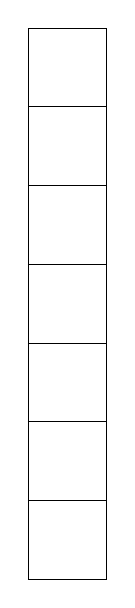
\begin{tikzpicture}
		\draw[step=1cm,black,very thin] (8,-0) grid (9,7);
	\end{tikzpicture}}

%\end{minipage}
%\end{document}
}}\hspace{0.5em}
	\subfloat[After \acrshort{MC} applied]{\label{fig:mc_problem_b} \scalebox{0.625}{%\end{minipage}
\def\rowperm{{0, 1, 2, 3, 4, 5, 6}}
%\def\colperm{{0, 1, 2, 3, 4, 5, 6}}
\def\colperm{{0, 1, 2, 3, 4, 5, 6}}
%\begin{minipage}{0.55\textwidth}
%\centering
\scalebox{0.7}{\begin{tikzpicture}
	\foreach \x in {0,1}
	\fill[red!65!white] (\colperm[\x]-1,6) rectangle (\colperm[\x],7);  
	\foreach \x in {0,1,2}
	\fill[red!65!white] (\colperm[2+\x]-1,5) rectangle (\colperm[2+\x],6);   
	\foreach \x in {0,1}
	\fill[red!65!white] (\colperm[5+\x]-1,4) rectangle (\colperm[5+\x],5); 

	\node at (\colperm[0]-0.5,6.5) {\Large{1}}; 
	\node at (\colperm[1]-0.5,6.5) {\Large{1}}; 
	\node at (\colperm[2]-0.5,5.5) {\Large{2}}; 
	\node at (\colperm[3]-0.5,5.5) {\Large{2}}; 
	\node at (\colperm[4]-0.5,5.5) {\Large{2}}; 
	\node at (\colperm[5]-0.5,4.5) {\Large{3}}; 
	\node at (\colperm[6]-0.5,4.5) {\Large{3}}; 
	
	\foreach \x in {0,1,2}
	\fill[green!65!white] (\colperm[\x]-1,3) rectangle (\colperm[\x],4);  
	\foreach \x in {0,1,2}
	\fill[green!65!white] (\colperm[3+\x]-1,2) rectangle (\colperm[3+\x],3);   
	\draw[step=1cm,gray,very thin] (-1,-0) grid (6,7);
	\node at (\colperm[0]-0.5,3.5) {\Large{1}}; 
	\node at (\colperm[1]-0.5,3.5) {\Large{1}}; 
	\node at (\colperm[2]-0.5,3.5) {\Large{1}}; 
	\node at (\colperm[3]-0.5,2.5) {\Large{2}}; 
	\node at (\colperm[4]-0.5,2.5) {\Large{2}}; 
	\node at (\colperm[5]-0.5,2.5) {\Large{2}}; 
	
	\foreach \x in {0,1,2}
	\fill[blue!65!white] (\colperm[1+\x]-1,1) rectangle (\colperm[1+\x],2);  
	\foreach \x in {0,1,2}
	\fill[blue!65!white] (\colperm[4+\x]-1,0) rectangle (\colperm[4+\x],1);
	\draw[step=1cm,gray,very thin] (-1,-0) grid (6,7);   
	
	\node at (\colperm[1]-0.5,1.5) {\Large{1}}; 
	\node at (\colperm[2]-0.5,1.5) {\Large{1}}; 
	\node at (\colperm[3]-0.5,1.5) {\Large{1}}; 
	\node at (\colperm[4]-0.5,0.5) {\Large{2}}; 
	\node at (\colperm[5]-0.5,0.5) {\Large{2}}; 
	\node at (\colperm[6]-0.5,0.5) {\Large{2}}; 
	\draw[step=1cm,black,very thin] (-1,-0) grid (6,7);
\end{tikzpicture}}
\hspace{0.3cm}
\scalebox{0.7}{\begin{tikzpicture}
	\foreach \x in {0,1,2,3,4,5,6}
	\fill[red!65!white] (8,\x) rectangle (9,\x+1);  
	\draw[step=1cm,black,very thin] (8,-0) grid (9,7);
	\node at (8.5,6.5-\colperm[0]) {\Large{1}}; 
	\node at (8.5,6.5-\colperm[1]) {\Large{1}}; 
	\node at (8.5,6.5-\colperm[2]) {\Large{2}}; 
	\node at (8.5,6.5-\colperm[3]) {\Large{2}}; 
	\node at (8.5,6.5-\colperm[4]) {\Large{2}}; 
	\node at (8.5,6.5-\colperm[5]) {\Large{3}}; 
	\node at (8.5,6.5-\colperm[6]) {\Large{3}}; 
\end{tikzpicture}}
%\end{minipage}
%\end{document}
}}
	%	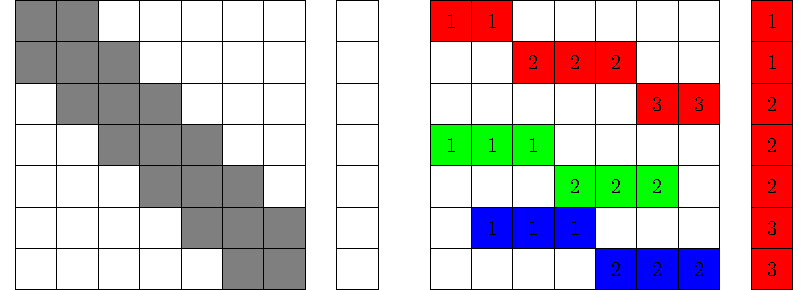
\includegraphics[scale=0.6]{pics/alpha_problem/mc_alpha_unsymm_only_red.tex}
	\caption{\label{fig:mc_problem} Illustration of data locality degradation due to \acrshort{MC}.
		Numbers represent thread id. Note that this figure shows only rows of matrix
		 permuted according to \acrshort{MC}, but in practice one would permute both 
		 rows and columns.}
\end{figure}
However this process comes at the cost of destroying data locality in the matrix by the required permutations. 
In the \acrshort{SymmSpMV} example (see \cref{alg:symmSpMV}) 
threads within a color operate on different rows having entirely different 
$col[idx]$ avoiding write conflicts in $b$ vector. 
%\Cref{fig:mc_problem}
%shows an illustration of a matrix before (\Cref{fig:mc_problem_a}) and 
%after (\Cref{fig:mc_problem_b}) applying \acrshort{MC} permutation.
Note, that within a color (for \eg red) none of the rows share same column index.
As the matrix is traversed row by row (see \cref{alg:symmSpMV}) the original matrix
has good data locality and most of the indirect vector accesses 
($x[col[idx]]$ and $b[col[idx]]$) correspond to nearby elements 
that were loaded in the computation of previous rows.
This ensures these vectors needs to be loaded only
once from main memory, and the rest of the accesses are served by 
fast caches. However coloring the matrix destroys this data locality. For example
in \Cref{fig:mc_problem_b} computing all the red colored rows leads to loading the 
entire vector completely. If the cache holds only  six elements, 
computation on green and blue rows require loading almost the entire vector again 
from the slow main memory.
\begin{figure}[b]
	\subfloat[Scaling performance]{\label{fig:motivation_symm_spmv}\scalebox{0.8}{\pgfplotsset{width=5.5cm,height=7.25cm,compat=1.3}
\def\matrixFile{pics/Spin-26/data}
\def\matrix{Spin-26}
\def\matrixName{Spin-26 }
\pgfplotstableread[col sep=comma] {\matrixFile/MKL/\matrix/spmv.txt} \SPMV
\pgfplotstableread[col sep=comma] {\matrixFile/MC_RCM/\matrix/symm_spmv.txt} \SYMMSPMVMC
\pgfplotstableread[col sep=comma] {\matrixFile/ABMC_RCM/\matrix/symm_spmv.txt} \SYMMSPMVABMC
\pgfplotstableread[col sep=comma] {\matrixFile/RACE/\matrix/symm_spmv.txt} \SYMMSPMVRACE
\pgfplotstableread[col sep=space] {\matrixFile/nnz} \NNZfile

\pgfplotstablegetelem{0}{nnz}\of\NNZfile
\pgfmathsetmacro{\NNZ}{\pgfplotsretval}

\newcommand{\rlmCopy}{7.627}
\newcommand{\rlmLoad}{8.962}
\begin{tikzpicture}[tight background]


\def\xmin{0}
\def\xmax{10}
\def\ymin{0}
\def\ymax{30}

\begin{axis}[ xlabel={Threads}, ylabel={Performance (GF/s)}, ymode=linear,
x tick label style={font={\Large}},
y tick label style={font={\Large}},
%xtick={1000, 2744, 5832, 10648, 17576, 27000, 39304, 54872, 74088},
%xticklabels={$10^3$, %$14^3$
%  , $18^3$, $22^3$, $26^3$, $30^3$, $34^3$, $38^3$, $42^3$},
scaled ticks=false,
%xmode=log,
xmin=0,xmax = 10,
ymin=0,
ymax=9.9,
%xlabel style={xshift=0.75em},
%ymin=0, ymax=14,
legend style={legend pos=north west, font=\footnotesize}]

%\addplot+[line width=2, color=magenta, mark options={magenta}] table[x =THREAD,y =PERF (GFlop/s),col sep=comma] {\SPMV}; \label{plot_one}
%\addlegendentry{SpMV}

\addplot+[line width=2, color=green, mark options={green}] table[x =THREAD,y =PERF (GFlop/s),col sep=comma] {\SYMMSPMVMC}; \label{plot_two}
\addlegendentry{SymmSpMV MC}

\addplot+[line width=2, color=cyan, mark options={cyan}] table[x =THREAD,y =PERF (GFlop/s),col sep=comma] {\SYMMSPMVABMC}; \label{plot_three}
\addlegendentry{SymmSpMV ABMC}

\addplot+[line width=2, color=orange, mark options={orange}] table[x =THREAD,y =PERF (GFlop/s),col sep=comma] {\SYMMSPMVRACE}; \label{plot_four}
\addlegendentry{SymmSpMV RACE}

%\addplot+[name path=RLM-copy, mark=square*, mark options={red}, draw=red] coordinates {(1,\rlmCopy) (6, \rlmCopy) (8, \rlmCopy) (10, \rlmCopy)}; \label{plot_five}
%\addlegendentry{Ideal}
  

\end{axis}
\end{tikzpicture}
}}\hspace{0.5em}
	\subfloat[Data traffic]{\label{fig:motivation_data}\scalebox{0.8}{\documentclass{standalone}
\usepackage{tikz}
\usepackage{pgfplots}
\pgfplotsset{width=15cm,height=12cm,compat=1.3}
\usepackage{filecontents}
\usetikzlibrary{patterns}
\usepackage{pgfplotstable}

\def\matrixFile{../data/}
\def\matrix{Spin-26}
\def\matrixName{Spin-26 }
\newcommand{\ideal}{11.25}

\begin{document}
	\pgfplotstableread[col sep=comma] {\matrixFile/MKL/\matrix/spmv.txt} \SPMV
	\pgfplotstableread[col sep=comma] {\matrixFile/MC_RCM/\matrix/spmv.txt} \SPMVMC
	\pgfplotstableread[col sep=comma] {\matrixFile/MC_RCM/\matrix/symm_spmv.txt} \SYMMSPMVMC
	\pgfplotstableread[col sep=comma] {\matrixFile/ABMC_RCM/\matrix/spmv.txt} \SPMVABMC
	\pgfplotstableread[col sep=comma] {\matrixFile/ABMC_RCM/\matrix/symm_spmv.txt} \SYMMSPMVABMC
	\pgfplotstableread[col sep=comma] {\matrixFile/RACE/\matrix/symm_spmv.txt} \SYMMSPMVRACE
	\pgfplotstableread[col sep=space] {\matrixFile/nnz} \NNZfile
		
	\pgfplotstablegetelem{0}{nnz}\of\NNZfile
	\pgfmathsetmacro{\NNZ}{\pgfplotsretval}
		
	
		\begin{tikzpicture}
		\begin{axis}[
		width  = 12cm,
		height = 11cm,
		major x tick style = transparent,
		minor ytick={1, 5, 10, 15, 20, 25, 30 ,35,40},
		grid = minor,
		ybar=2*\pgflinewidth,
		bar width=16pt,
		ymajorgrids = true,
		grid style={dashed, gray!40},
		ylabel = {\Large{Bytes/NNZ}},
		symbolic x coords={SpMV, SymmSpMV-MC, SymmSpMV-ABMC},
		x tick label style={rotate=25,font={\large}},
		y tick label style={font={\Large}},
		xtick = data,
		scaled y ticks = false,
		enlarge x limits=0.25,
		ymin=0,% ymax=42,
		legend cell align=left,
		legend style={
			%at={(1,1.05)},
			%anchor=south east,
			%column sep=1ex,
			legend pos=north west
		},
		]
		

		\pgfkeys{/pgf/fpu}

		\pgfplotstablegetelem{9}{MEM (GB)}\of\SPMV
		\pgfmathsetmacro{\memSPMV}{\pgfplotsretval*1*1/(\NNZ*0.5*1e-8)} %change to SpMV
		\pgfplotstablegetelem{9}{MEM (GB)}\of\SPMVMC
		\pgfmathsetmacro{\memSPMVMC}{\pgfplotsretval*1*1/(\NNZ*0.5*1e-8)}
		\pgfplotstablegetelem{9}{MEM (GB)}\of\SPMVABMC
		\pgfmathsetmacro{\memSPMVABMC}{\pgfplotsretval*1*1/(\NNZ*0.5*1e-8)}
		\pgfplotstablegetelem{9}{MEM (GB)}\of\SYMMSPMVMC
		\pgfmathsetmacro{\memSYMMSPMVMC}{\pgfplotsretval*1*1/(\NNZ*0.5*1e-8)}
		\pgfplotstablegetelem{9}{MEM (GB)}\of\SYMMSPMVABMC
		\pgfmathsetmacro{\memSYMMSPMVABMC}{\pgfplotsretval*1*1/(\NNZ*0.5*1e-8)}
		\pgfplotstablegetelem{9}{MEM (GB)}\of\SYMMSPMVRACE
		\pgfmathsetmacro{\memSYMMSPMVRACE}{\pgfplotsretval*1*1/(\NNZ*0.5*1e-8)}
		
		\addplot[pattern=horizontal lines]%style={ppurple,fill=ppurple}]
		coordinates {(SpMV,\memSPMV) (SymmSpMV-MC,\memSYMMSPMVMC) (SymmSpMV-ABMC,\memSYMMSPMVABMC)};

		\pgfplotstablegetelem{9}{L3 (GB)}\of\SPMV
		\pgfmathsetmacro{\memSPMV}{\pgfplotsretval*1*1/(\NNZ*0.5*1e-8)} %change to SpMV
		\pgfplotstablegetelem{9}{L3 (GB)}\of\SPMVMC
		\pgfmathsetmacro{\memSPMVMC}{\pgfplotsretval*1*1/(\NNZ*0.5*1e-8)}
		\pgfplotstablegetelem{9}{L3 (GB)}\of\SPMVABMC
		\pgfmathsetmacro{\memSPMVABMC}{\pgfplotsretval*1*1/(\NNZ*0.5*1e-8)}
		\pgfplotstablegetelem{9}{L3 (GB)}\of\SYMMSPMVMC
		\pgfmathsetmacro{\memSYMMSPMVMC}{\pgfplotsretval*1*1/(\NNZ*0.5*1e-8)}
		\pgfplotstablegetelem{9}{L3 (GB)}\of\SYMMSPMVABMC
		\pgfmathsetmacro{\memSYMMSPMVABMC}{\pgfplotsretval*1*1/(\NNZ*0.5*1e-8)}
		\pgfplotstablegetelem{9}{L3 (GB)}\of\SYMMSPMVRACE
		\pgfmathsetmacro{\memSYMMSPMVRACE}{\pgfplotsretval*1*1/(\NNZ*0.5*1e-8)}

		\addplot[fill=gray!180]%style={ppurple,fill=ppurple}]
		coordinates {(SpMV,\memSPMV) (SymmSpMV-MC,\memSYMMSPMVMC) (SymmSpMV-ABMC,\memSYMMSPMVABMC)};

		\pgfplotstablegetelem{9}{L2 (GB)}\of\SPMV
		\pgfmathsetmacro{\memSPMV}{\pgfplotsretval*1*1/(\NNZ*0.5*1e-8)} %change to SpMV
		\pgfplotstablegetelem{9}{L2 (GB)}\of\SPMVMC
		\pgfmathsetmacro{\memSPMVMC}{\pgfplotsretval*1*1/(\NNZ*0.5*1e-8)}
		\pgfplotstablegetelem{9}{L2 (GB)}\of\SPMVABMC
		\pgfmathsetmacro{\memSPMVABMC}{\pgfplotsretval*1*1/(\NNZ*0.5*1e-8)}
		\pgfplotstablegetelem{9}{L2 (GB)}\of\SYMMSPMVMC
		\pgfmathsetmacro{\memSYMMSPMVMC}{\pgfplotsretval*1*1/(\NNZ*0.5*1e-8)}
		\pgfplotstablegetelem{9}{L2 (GB)}\of\SYMMSPMVABMC
		\pgfmathsetmacro{\memSYMMSPMVABMC}{\pgfplotsretval*1*1/(\NNZ*0.5*1e-8)}
		\pgfplotstablegetelem{9}{L2 (GB)}\of\SYMMSPMVRACE
		\pgfmathsetmacro{\memSYMMSPMVRACE}{\pgfplotsretval*1*1/(\NNZ*0.5*1e-8)}
				
		\addplot[pattern=vertical lines]%style={ppurple,fill=ppurple}]
		coordinates {(SpMV,\memSPMV) (SymmSpMV-MC,\memSYMMSPMVMC) (SymmSpMV-ABMC,\memSYMMSPMVABMC)};
	
		
		\pgfkeys{/pgf/fpu=false}

		\addplot[draw=red,smooth,dashed, line width=3pt] coordinates { (SymmSpMV-MC,\ideal) (SymmSpMV-ABMC,\ideal)};
				
		\legend{MEM, L3, L2, Ideal SymmSpMV}
		\end{axis}
	%	\node at (6.5,10) {Data traffic Comparison using LIKWID};
		\end{tikzpicture}
\end{document}
}}
	\caption{\label{fig:motivation}(a) Performance of \acrshort{SymmSpMV} with 
		\acrshort{MC} and \acrshort{ABMC} compared to \acrshort{RACE}. 
		(b) Average main memory data traffic in bytes (B) per nonzero entry ($\acrshort{nnz}$) 
		of the full matrix as measured with \LIKWID tool \cite{LIKWID}. The ideal data traffic
		as predicted by performance model is shown for reference.}
\end{figure}


%The matrix after multicoloring permutation is seen in \Cref{fig:mc_problem_b},
%observe that within a color (for \eg red) none of the rows share same column entry. 
%Traversing the elements of the original matrix row by row, would require only 
%one time loading of the right-hand-side (RHS) vector entry, as the elements 
% carried out on
% a matrix (see \Cref{fig:mc_problem_a}) that initially has high data locality.
Destroying data locality along with secondary effects like 
synchronization costs and false sharing may, thus lead to severe performance degradation for MC methods.
We demonstrate the impacts on performance and 
data transfer volumes for the \acrshort{SymmSpMV} computations in ~\Cref{fig:motivation} for a single 10-core  \Intel \IVB (E5-2660 v2) CPU clocked at 2.2\,\GHZ.
The experiment was done on a large (number of rows $= 10400600$) \texttt{Spin-26} \cite{Spin} matrix taken from quantum physics application. 
We find that performance of MC methods scale decently within a socket but are far off the RACE performance which saturates main memory bandwidth at 6-7 cores (~\Cref{fig:motivation_symm_spmv} ).
The reason for the large performance difference is given in \Cref{fig:motivation_data} which shows the average main memory data traffic per non-zero  of the 
general matrix during \acrshort{SymmSpMV} execution. It can be clearly seen that 
the memory traffic is almost  $4 \times$ higher 
for the \acrshort{MC} method compared to ideal traffic (red line) predicted
by an appropriate performance model\footnote{See \Cref{sec:results} for more details on modeling.}.
The extra data traffic is mainly due to the low data locality and thereby incurred 
extra accesses of the indirectly accessed vectors. 
\Acrfull{ABMC} tries to reduce the memory traffic by first partitioning the matrix
into blocks and then applying coloring. This improves (reduces) the data traffic compared 
to \acrshort{MC} but is still far from optimal in this case. 

%\underline{}
As main memory bandwidth is the main bottleneck on modern compute devices,
 this extra traffic reflects directly on the performance.
This is seen in \Cref{fig:motivation_symm_spmv}, where the performance is
shown in giga floating point operations in seconds (\GF). The ideal 
 performance as predicted by performance model is $\approx 7.6\,\GF$ (not shown in figure)
 for this matrix, but \acrshort{MC} and \acrshort{ABMC} are well below this limit.
 However our \acrshort{RACE} method closely approaches the ideal values both for
 the data traffic and performance and provides a speed-up 
of almost  $4\times$ compared to other methods.

\begin{comment}
\Cref{fig:motivation_symm_spmv} shows performance in giga floating point 
operations per second (\GF) as a function of thread (core).
The general variant  of sparse matrix-vector multiplication (\acrshort{SpMV})
 using the full matrix  serves as the yardstick for comparison. 
Based on a naive performance analysis, as most of the sparse
kernels are highly memory bound on modern architectures
one would expect \acrshort{SymmSpMV} performance 
to be almost twice that of \acrshort{SpMV}, due to half the data traffic. 
However the \acrshort{SymmSpMV} implementation using \acrshort{MC} is more
than three times slower.
\end{comment}

\section{RACE Method} \label{sec:RACE_method}
\acrshort{RACE} was designed with the shortcomings
of coloring approaches in mind. The idea is to have a general hard\-ware-friendly
approach applicable even for simple matrix storage formats 
like \acrshort{CRS}.
The \Acrshort{RACE} method consists of three steps: (1) level construction,
(2) \DK coloring, and (3) load balancing.
Depending on the matrix and hardware the steps are applied recursively 
if required. 
To illustrate the method we choose a
simple matrix which is associated with an artificially constructed
two-dimensional-seven-point (2d-7pt) stencil. \Cref{fig:orig_graph} shows
the corresponding graph and the sparsity pattern (see inset) of the matrix.
In this paper we restrict ourselves to matrices representing strongly connected 
undirected graphs.

\subsection{Level Construction}
In the first step we determine the levels of a graph and permute the data structure accordingly.
Here, we  use well-known bandwidth reduction algorithms like \Acrfull{RCM}\cite{RCM}
or \Acrfull{BFS}\cite{BFS}. Although \acrshort{RCM} is implemented in \acrshort{RACE},
in the following we apply \acrshort{BFS} reordering for better illustration.
% \setlength{\belowcaptionskip}{0pt}
\begin{figure}[tb]
	\subfloat[Original graph]{\label{fig:orig_graph}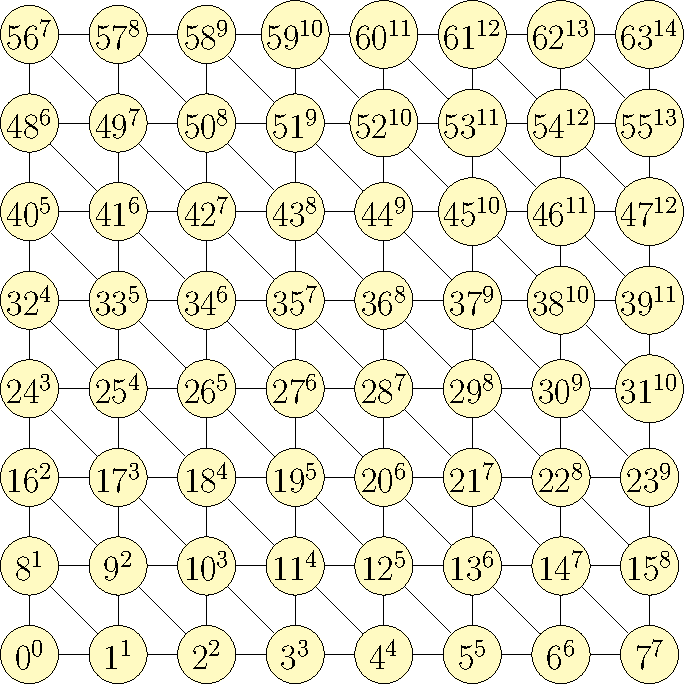
\includegraphics[scale=0.32]{pics/race_method/orig_graph}
		\begin{picture}(0,0)
		\put(-42.5,65.5){{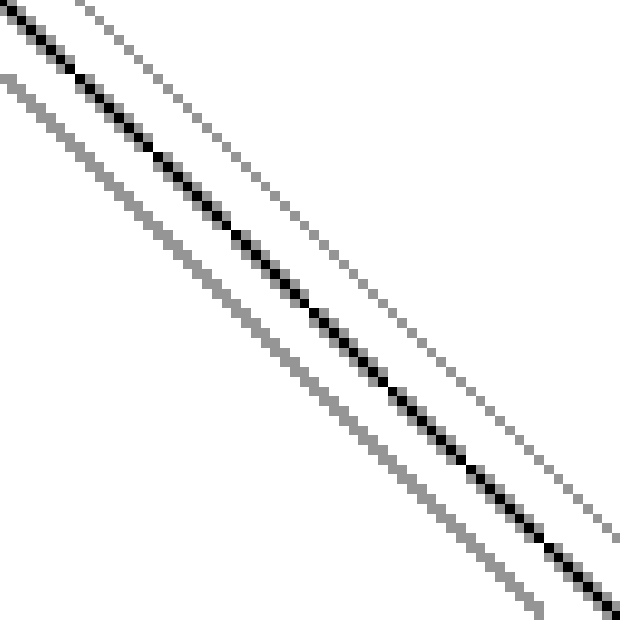
\includegraphics[scale=0.065]{pics/race_method/orig_matrix}}}
		\end{picture}
	}
	\subfloat[Permuted graph]{\label{fig:perm_graph}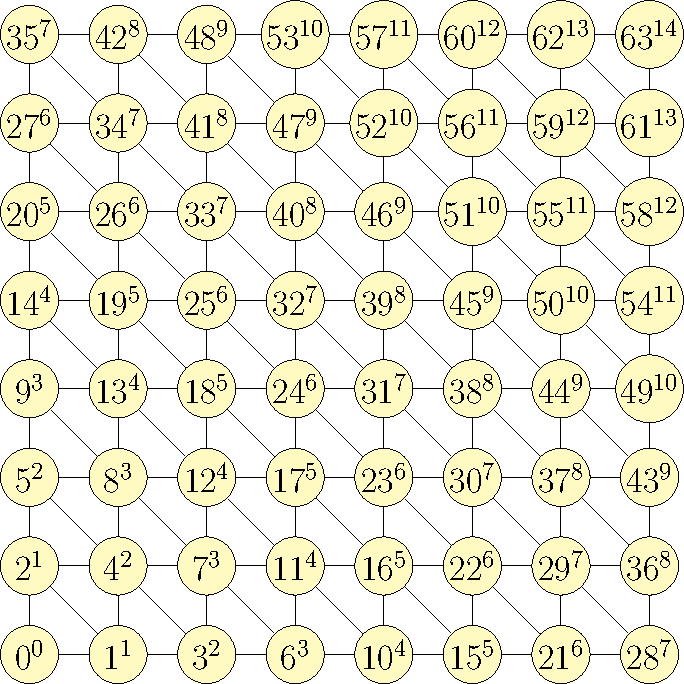
\includegraphics[scale=0.32]{pics/race_method/perm_graph}
		\begin{picture}(0,0)
		\put(-42.5,65.5){{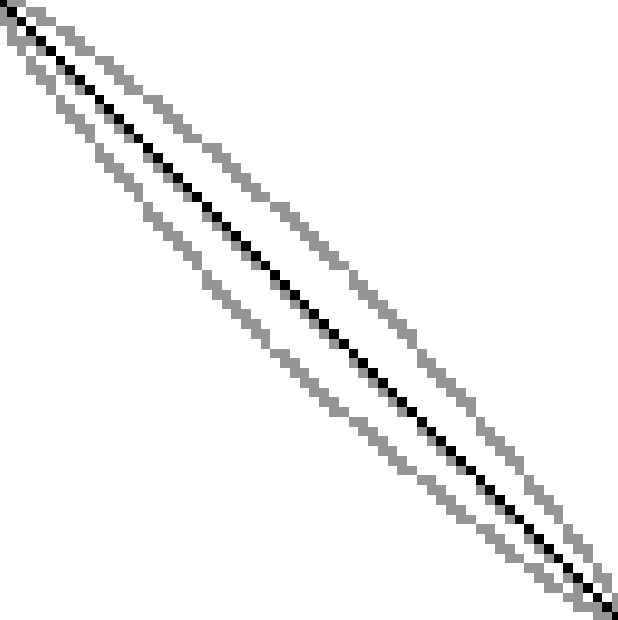
\includegraphics[scale=0.065]{pics/race_method/perm_matrix}}}
		\end{picture}
	}
	\subfloat[]{\label{fig:levelPtr}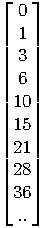
\includegraphics[scale=0.95]{pics/race_method/levelPtr}
		}
	\caption{\label{fig:level_construction}(a) Original graph of the 2d-7pt example, domain size $8 \times 8$. (b) Graph after permutation according to levels. The level numbers are denoted on the superscript of the vertices. Figures in inset show the corresponding sparsity pattern of the matrix. (c) \levelPtr}
\end{figure}
We start with choosing a root vertex and assign it to the first level ($L(0)$). 
The next levels $L(i)$ are defined to contain all vertices that are directly related to the previous
level $L(i-1)$ but are not in $L(i-2)$. This implies that the $i$-th level consists of all vertices
that have a minimum distance of $i$ from the root node. In \Cref{fig:level_construction} the
level numbers ($i$) are denoted in the superscript of the vertices. 

After the levels are determined we permute (reorder) the matrix (and graph) according
to the levels such that the vertices in $L(i)$ appear before $L(i+1)$.  \Cref{fig:perm_graph}
shows the graph and matrix after applying the permutation. Note that the vertex numbering 
in the permuted graph has changed compared to the original lexicographically ordered
matrix.
It is well known  that such a permutation improves data locality,
and it was previously applied to sparse matrix
computations without dependencies \cite{RCM_Sparse_computation}.

\Inorder to resolve dependencies, \acrshort{RACE} additionally keeps information
about the levels by storing the index of the first vertex corresponding
to each level in a data structure called \levelPtr (see \Cref{fig:levelPtr}).

\subsection{Distance-k Coloring}
The \DK coloring step uses the information of the \levelPtr to resolve
dependencies. Two vertices are called \DK neighbors if the shortest path connecting 
them consists of at most $k$ edges \cite{dist_k_def}. This implies two vertices
 are \DK independent if they are not \DK neighbors. Based on this definition
 it can be proven that vertices between levels $L(i)$ and $L(i \pm (k+j))$ are
 \DK independent $\forall j\ge1$. The levels that satisfy this criterion
 are called \DK independent levels.
 
 %\setlength{\belowcaptionskip}{-8pt}
 \begin{figure}[t]
 	\vspace*{-0.6cm}
 	\subfloat[\DONE coloring]{\label{fig:d1_color}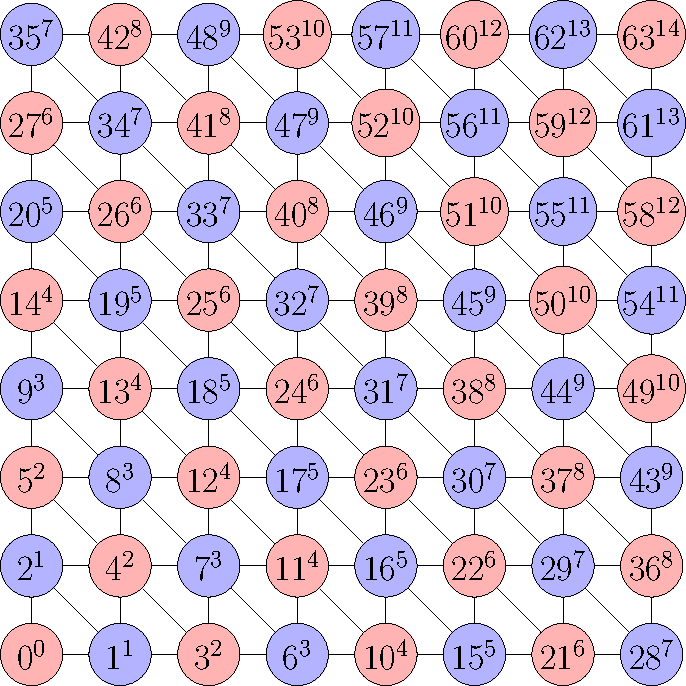
\includegraphics[scale=0.32]{pics/race_method/d1_color}}
 	\subfloat[\DTWO coloring]{\label{fig:d2_color}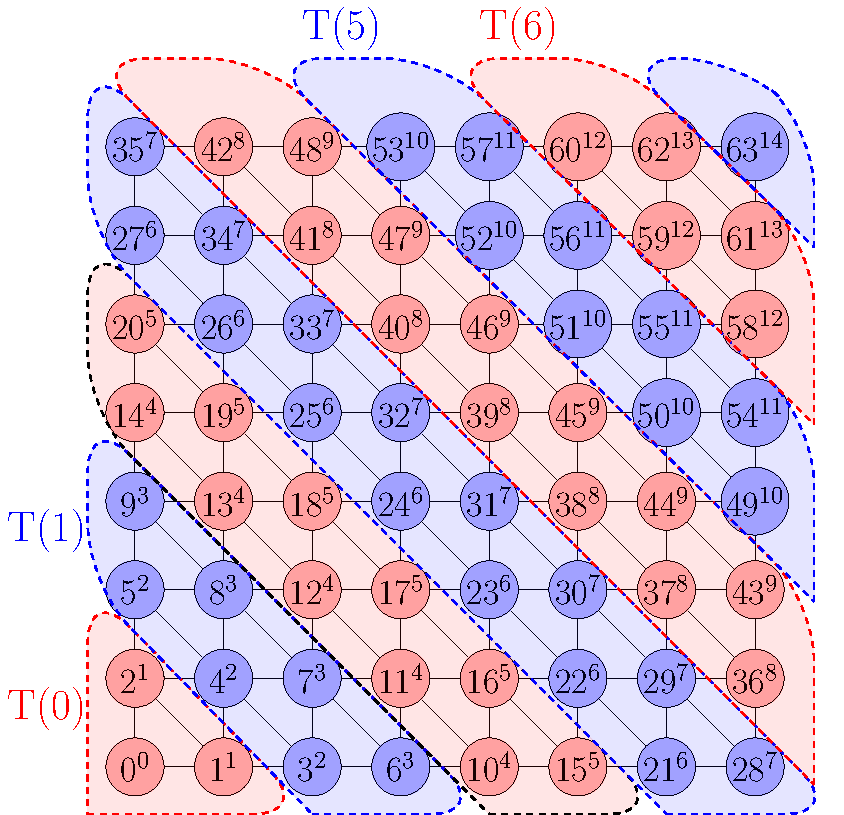
\includegraphics[scale=0.32]{pics/race_method/d2_color}}
 	\caption{\label{fig:dk_color} Example of \DONE and \DTWO coloring of the matrix shown in \Cref{fig:level_construction}}
 \end{figure}
 % \setlength{\belowcaptionskip}{0pt}
The above approach allows for many choices to form \DK independent levels. \Cref{fig:dk_color} shows 
one such possibility for \DONE and \DTWO coloring each. As $L(i)$ and $L(i\pm2)$ are
distance-1 independent, the \DONE coloring  assigns
two colors to alternating levels.  In case of \DTWO we group two adjacent levels and apply \DONE
coloring to the groups. These groups of levels are called \levelGroups
 and the $i-th$ \levelGroup is denoted as $T(i)$ (see \Cref{fig:d2_color}).
For \DONE coloring shown in \Cref{fig:d1_color} the \levels and \levelGroups
coincide ($L(i) = T(i)$).
In both cases
 all the vertices  between \levelGroups of same color
  are \DONE/\DTWO independent  and can be executed in parallel.
   For example, in case of \DTWO, \levelGroups $T(0), T(2), T(4)$
 and $T(6)$ can be executed by four threads in parallel. After synchronization the remaining 
 four blue \levelGroups can be executed in parallel. Note that
 within a \levelGroup/\level the vertices are computed serially without destroying
 any data locality.

Choosing the same number of \levels per \levelGroup may cause severe
load imbalance depending on the matrix. For example, in \Cref{fig:d2_color} 
 \levelGroups at extreme ends $T(0), T(7)$  have a relatively low number of 
 vertices (proportional to computational work)  compared to the \levelGroups 
 in the middle ($T(3),T(4)$).


\subsection{Load Balancing}
\Acrshort{RACE} applies a load-balancing scheme 
among the threads within each color.
%The main idea 
%is to include hardware features like number of threads into the 
%method.
It generates just the right number of \levelGroups 
as required by the hardware (i.e., the number of available threads)
and then applies a load-balancing algorithm that
minimizes the variance among the number of vertices 
within \levelGroups of the same color. To this end,
\levelGroups containing few vertices
grab adjacent \levels from neighboring \levelGroups; overloaded
\levelGroups shift \levels to adjacent \levelGroups. To maintain
\DK independence between \levelGroups of the same color the algorithm enforces \atleast $k$ levels per \levelGroup. This shifting process is applied iteratively until it
reaches the minimum possible variance or no further moves are possible due to
 \DK coloring.
 
%  \setlength{\belowcaptionskip}{-10pt}
  \begin{figure}[t]
  	\begin{minipage}[c]{0.26\textwidth}
  	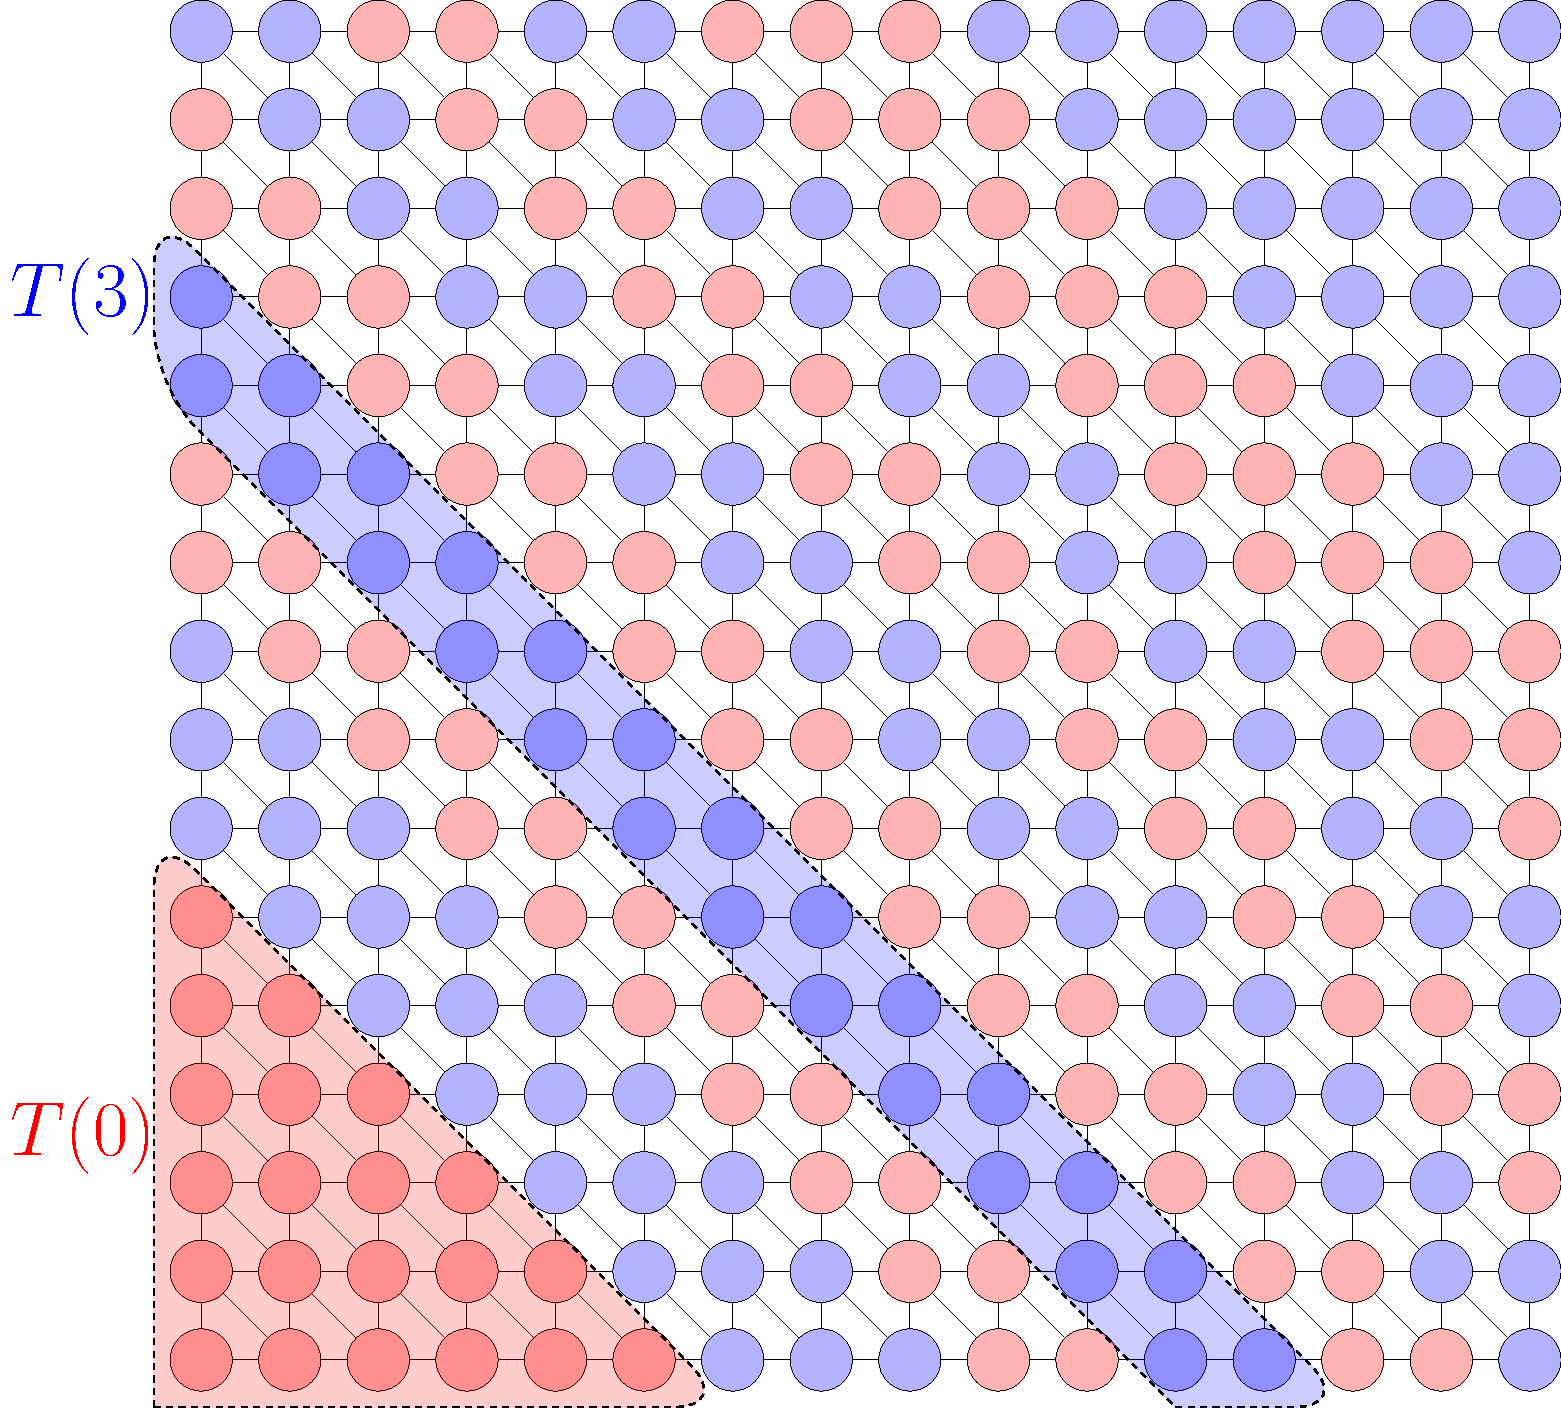
\includegraphics[height=12.4em,width=15.2em]{pics/race_method/load_balancing}
  	\end{minipage}\hspace{2.2em}
  	 \begin{minipage}[c]{0.16\textwidth}
  	\caption{\label{fig:lb} Applying load balancing for five threads and resolving \DTWO
  		dependency for the 2d-7pt example from ~\Cref{fig:level_construction} but now with domain size $16\times16$.  }
  	\end{minipage}
  \end{figure}
%   \setlength{\belowcaptionskip}{0pt}
   
  \Cref{fig:lb} shows the graph of the 2d-7pt example at size $16\times16$ after
   load balancing. Here \DTWO coloring and five threads
    (\ie ten \levelGroups) were the input to the load balancer.
    Note that \levelGroups at extreme ends (\eg $T(0)$) have more levels
    since here each level has fewer vertices, whereas bigger \levelGroups
    (\eg $T(3)$) in the middle maintain two levels to preserve \DK coloring.
    
\subsection{Recursion}
However, using the steps above the generated parallelism is limited by the total number
of \levels, and the load balancing can be a problem as it gets closer to this limit.
To match the high levels of parallelism of modern compute devices  we use recursion. The formulation of \acrshort{RACE} allows to simply select a \levelGroup (sub-graph) and apply the three
 steps recursively on this sub-graph to exploit the parallelism 
 within this \levelGroup. The thread that was originally assigned to the
 \levelGroup spawns other parallel threads in a nested manner. 
 The selection of the \levelGroup to be used for recursion and final load balancing 
 is done by  a global load balancing algorithm.
 
 
\section{Results \& Contribution} \label{sec:results}
We evaluate the performance of \acrshort{RACE} by parallelizing the \acrshort{SymmSpMV}
kernel shown in \Cref{alg:symmSpMV}. This allows a clear picture of the
performance advantage of \acrshort{RACE}. Finally,
 we use \acrshort{RACE} to parallelize an eigenvalue solver, 
and compare against standard approaches.

\subsection{Analysis of SymmSpMV Performance} \label{subsec:perf_symm_spmv}
Matrix-vector multiplication is frequently used in
numerical algorithms. In many cases, however, 
the lack of an efficient and generic \acrshort{SymmSpMV} implementation
leads to the full (general) matrix being stored and used even if it is
symmetric, which wastes not only CPU cycles but also memory.
Modern HBM (High Bandwidth Memory) technology with its rather limited
memory sizes makes this problem even more severe. 

In this section we carry out experiments using a \acrshort{SymmSpMV} kernel.
We choose most of the test matrices from the public SuiteSparse Matrix Collection \cite{UOF}, 
that are frequently used in related publications \cite{RSB,park_ls}, as well as
some from the quantum physics context 
in which \acrshort{RACE} was developed \cite{ESSEX}.
The experiments are
run on one \Intel \SKX Gold 6148 CPU ($20$ threads) at a fixed clock speed of
2.4 \GHZ. The reported performance is purely for the \acrshort{SymmSpMV}
computation as in practical applications these kernels are called multiple times, 
making other costs (like setup time) negligible.

\begin{figure*}[tb]
	\subfloat[Performance of \acrshort{RACE} compared with MKL ]{\label{fig:race_vs_mkl}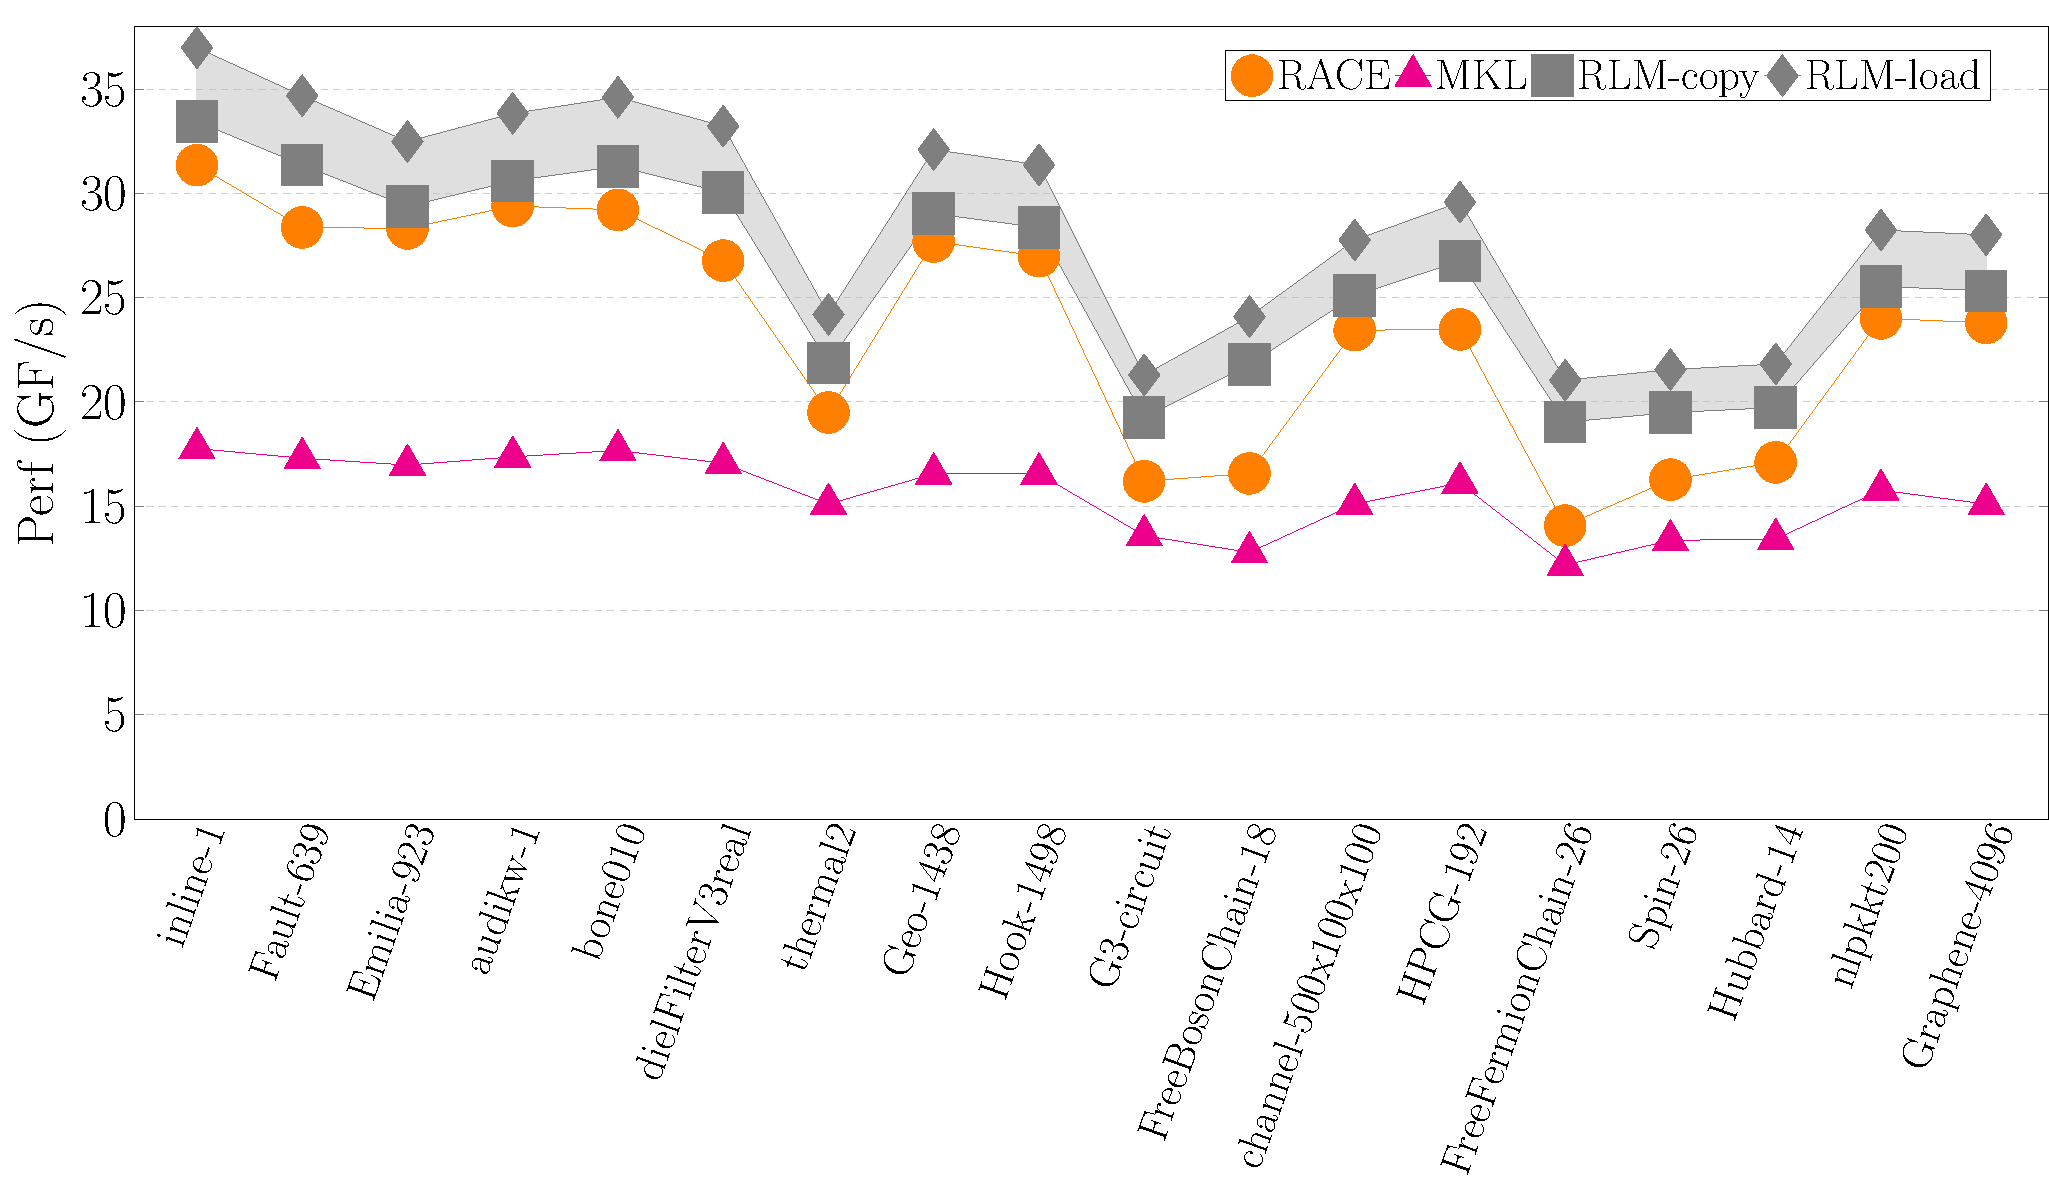
\includegraphics[scale=0.26]{pics/symm_spmv/skx/RACE_vs_MKL}}
	\subfloat[Performance of RACE compared to coloring approaches]{\label{fig:race_vs_mc}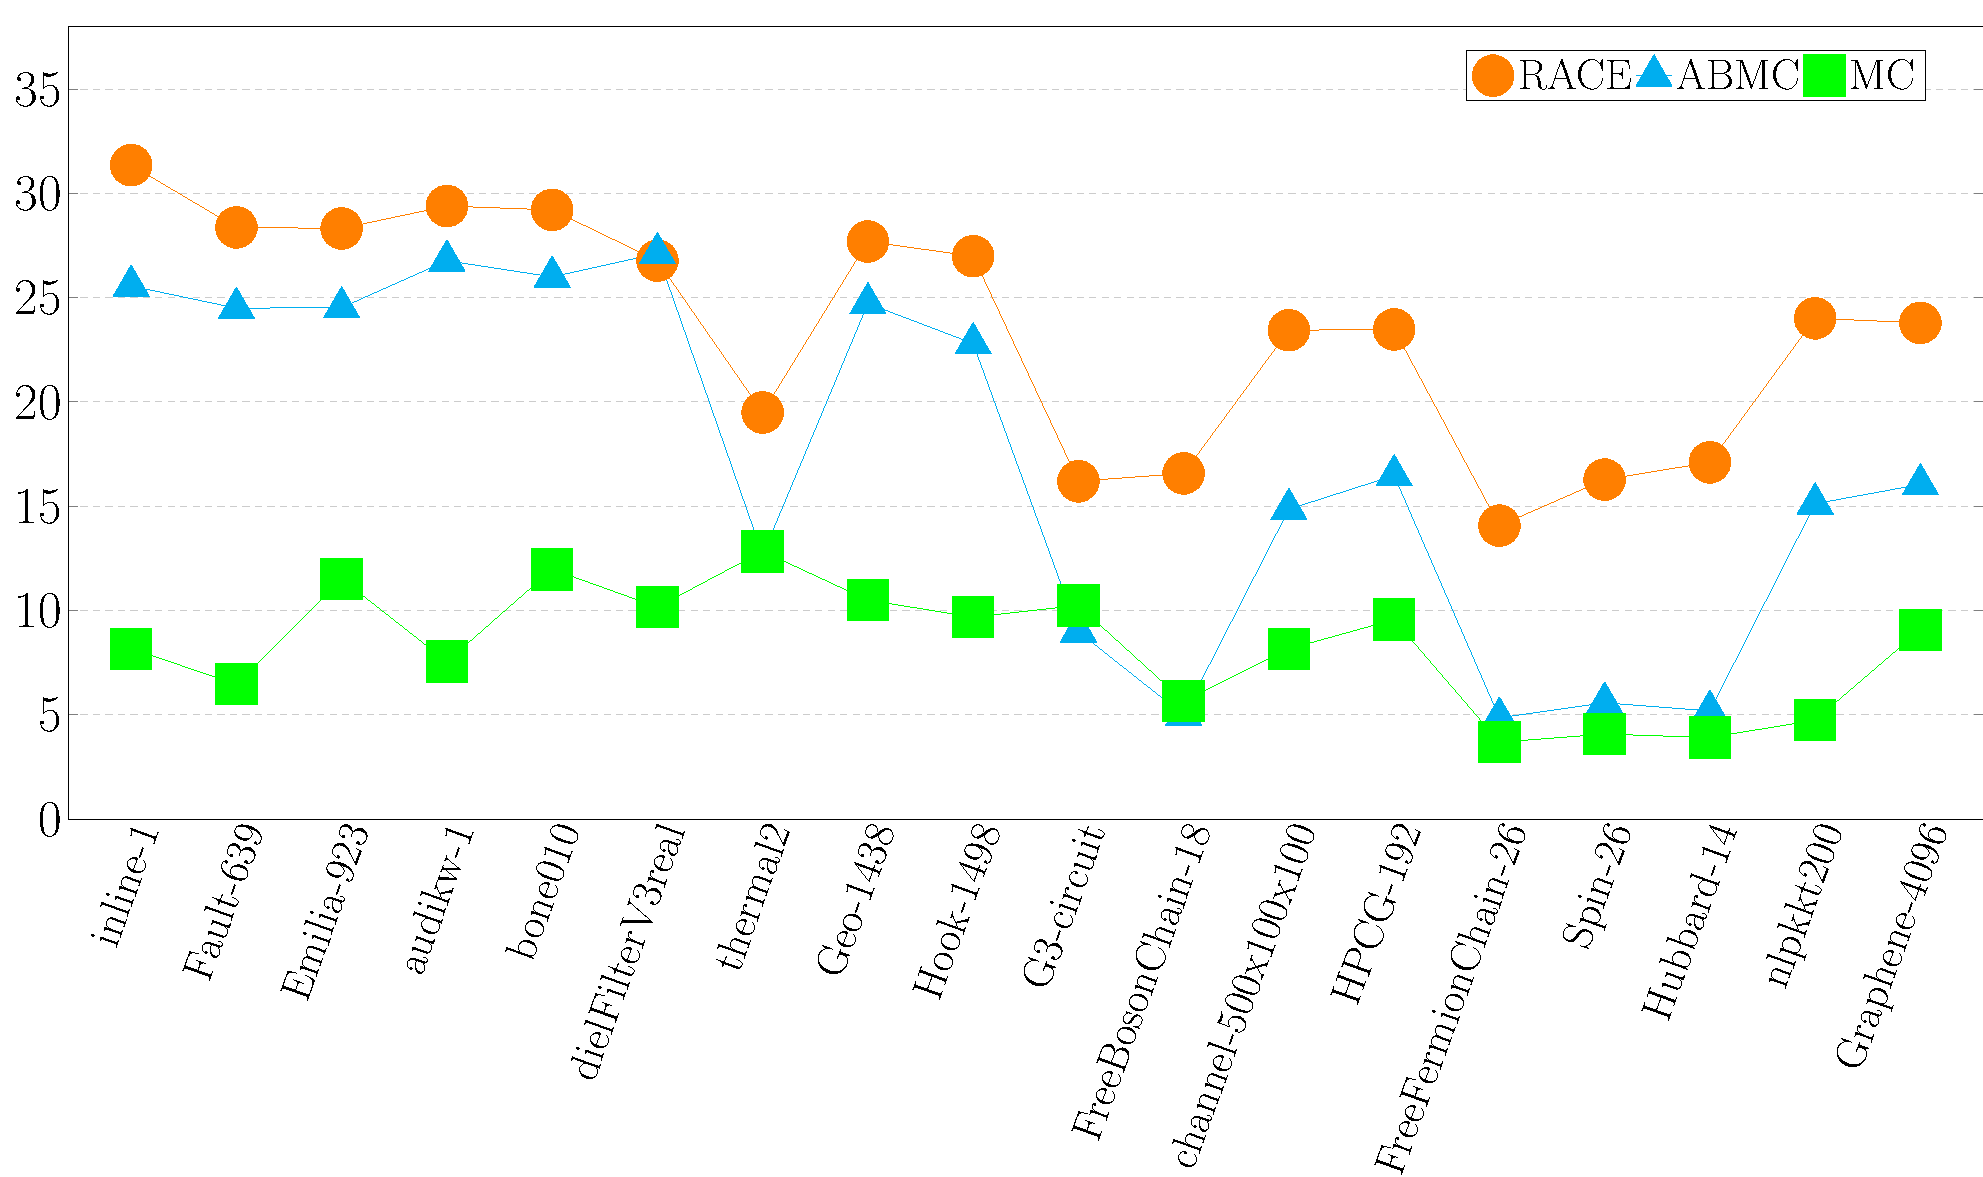
\includegraphics[scale=0.26]{pics/symm_spmv/skx/RACE_vs_MC}}
	\caption{\label{fig:symm_spmv_perf} \acrshort{SymmSpMV} performance of \acrshort{RACE} compared to 
		other methods. The Roof{}line model for \acrshort{SymmSpMV} is shown in 
		\cref{fig:race_vs_mkl} for reference. Note that the matrices are ordered according 
		to increasing number of rows.}
\end{figure*}
To establish a sensible performance baseline we use the Roof{}line  model (RLM)
\cite{Williams_roofline} along the lines of \cite{Moritz_sell} but adjusted
for the \acrshort{SymmSpMV} kernel. \Cref{fig:race_vs_mkl} shows the performance of \acrshort{RACE}
on different matrices along with the range of upper performance bounds based on two saturated memory bandwidth measurements (RLM-load and RLM-copy). 
In almost all cases, \acrshort{RACE} attains more than $85\%$ of the possible maximum. 
This can be attributed to the good data locality and minimal data traffic, which we have already demonstrated in \Cref{fig:motivation_data} for the \texttt{Spin-26} matrix. 
 
%Next we compare the \acrshort{RACE} method with other approaches. 
In \Cref{fig:race_vs_mkl} we compare against the \acrshort{SymmSpMV} 
implementation of the latest version of \acrshort{MKL} \cite{MKL},
which uses the Inspector-Executor routines.
The comparisons show that \acrshort{RACE} outperforms MKL
by a factor of $1.5\times$ on an average. 
A simple analysis
shows that the performance of the \acrshort{MKL} \acrshort{SymmSpMV} 
kernel coincides with the matrix-vector multiplication using the full
matrix (\acrshort{SpMV}). We can only speculate (due to it being closed source) that MKL converts
the symmetric matrix to a full matrix internally and then does a general \acrshort{SpMV} operation.
%However, MKL being closed source  the algorithm and the underlying 
%kernel is unknown.

We also compare \acrshort{RACE} with two widely used
coloring methods, \acrshort{MC} and \acrshort{ABMC}.
For \acrshort{MC} we apply the \acrlong{MC} scheme
generated by the COLPACK \cite{COLPACK} library to parallelize the \acrshort{SymmSpMV}
kernel. In the \acrshort{ABMC} method we first partition the matrix into blocks
using METIS \cite{METIS} and then apply coloring via \COLPACK. The
size of blocks was determined by a parameter scan (range 4 \ldots 128, see \cite{ABMC}).
\Cref{fig:race_vs_mc} shows the resulting performance data. 
Overall the \acrshort{MC} method is not competitive, while \acrshort{ABMC} delivers
modest performance ($85\%$ of \acrshort{RACE}) for small matrices. For large
matrices,  however, where data locality plays a vital role, \acrshort{ABMC} 
falls substantially behind \acrshort{RACE} as the indirect access to the vectors
impairs temporal and spatial access locality.
%GHa: Not necessary if there's no deeper discussion
%To make this comparison easier
%the matrices are arranged according to increasing number of rows.
Overall, \acrshort{RACE} shows an average speedup of $1.6\times$ compared to 
\acrshort{ABMC}, while in some cases the speedup is as high as $3\times$.


%First we establish performance model for 
%\acrshort{SymmSpMV} and compare it to \acrshort{RACE} performance to estimate
%the quality of our method. Then we compare \acrshort{RACE} with the
%two coloring approaches introduced before and the 



\subsection{FEAST with RACE}
FEAST\cite{FEAST} is a modern algorithm to compute inner eigenvalues.
It uses contour integration to generate a subspace (reduced system) containing the eigenvalues,
which are then solved using a classic Rayleigh-Ritz procedure. The solver is
well-suited for very large sparse systems, and is of particular interest in the field
of quantum mechanics.
 The hot spot of the algorithm (more than $95\%$) is a solver for
 shifted linear systems ($A- \sigma I = b$). These systems are, however, highly %indefinite
 %\GHcomm{is ``indefinite'' the right word here? If in doubt, stick with ``ill-conditioned''} and
 ill-conditioned, posing severe convergence
 problems for most linear iterative solvers. The standard approach
 is therefore to use direct solvers. However, in \cite{feast_mc} it has been shown
 that the Kaczmarz iterative solver accelerated by a Conjugate Gradient (CG) method
 (the  so-called CGMN solver \cite{cgmn}) is a robust alternative to direct solvers. 
Similar to \acrshort{SymmSpMV}, the Kaczmarz method has a \DTWO dependency, making
it difficult to parallelize. In \cite{feast_mc}, \acrlong{MC} was used to
parallelize the kernel. We have implemented a shared-memory parallel version of CGMN with \acrshort{RACE} for use in FEAST.

%  \setlength{\belowcaptionskip}{-15pt}
\begin{figure}[b]
	\centering
	\subfloat[\label{fig:feast_time}Time to solution]{\scalebox{0.57}{%\documentclass{standalone}
%\usepackage{tikz}
%\usepackage{pgfplots}

%\usepackage{comment}
%\usepackage{filecontents}

\pgfplotsset{width=7.5cm,height=8.75cm,compat=1.3}
%\begin{filecontents}{data_mkl.dat}
%size, nrows,   Time,		Mem		
%40,		64000,	9.92,		968724
%60,		216000,	76.31,	2739456
%70,		343000,	 230.26,	5066384 
%80,		512000, 452.685, 7670076
%120,	1728000, 6600.29, 36152256
%140, 	2744000, 16473.6, 65311968
%\end{filecontents}

%\begin{filecontents}{data_cgmn.dat}
%size, nrows,   Time,		Mem		
%40,		64000,	78.99,	332364
%60,		216000,	1007,  661684
%70,		343000,	 2277.09,  959544
%80,		512000, 4302.18, 1440628
%120,	1728000, 29777.8, 4106652
%140, 	2744000, 57916.9, 6316176
%160,	4096000, 118008, 9379604
%220,	10648000, 527629.5, 23632788
%\end{filecontents}


%\begin{document}

\begin{tikzpicture}


  \def\xmin{0}
  \def\xmax{10}
  \def\ymin{0}
  \def\ymax{30}

  \begin{axis}[ xlabel={Size (n)}, ylabel={Time(s)}, ymode=linear,
  xtick={ 64000, 125000, 216000, 512000,   1728000, 5832000, 15625000 },
  xticklabels={$40^3$
    , $50^3$, $60^3$,  $80^3$,   $120^3$, $180^3$, $250^3$ },
  ytick={ 100, 1000, 10000, 100000,   1000000},
  yticklabels={$10^2$
  	, $10^3$, $10^4$,  $10^5$,   $10^6$ },
  scaled ticks=false,
  xmode=log,
  ymode=log,
  ymax=100000000,
 % xmin=27000,xmax = 15625000,
  %ymin=0, ymax=14,
  legend style={legend pos=north west}]

   \addplot+[mark=square*, mark size=2pt, mark options={magenta}, draw=magenta, line width=1.5] table[x expr=\thisrow{size}*\thisrow{size}*\thisrow{size},y expr=\thisrow{Time},col sep=comma] {pics/feast/skx/data_mkl.dat}; \label{plot_one}
   \addlegendentry{Intel MKL(Pardiso)}

   \addplot+[mark=*, mark size=2pt, mark options={orange}, draw=orange, line width=1.5] table[x expr=\thisrow{size}*\thisrow{size}*\thisrow{size},y expr=\thisrow{Time},col sep=comma] {pics/feast/skx/data_cgmn.dat}; \label{plot_two}
   \addlegendentry{RACE-CGMN}

	\addplot+[mark=triangle*, mark size=2pt, mark options={cyan}, draw=cyan, line width=1.5 ] table[x expr=\thisrow{size}*\thisrow{size}*\thisrow{size},y expr=\thisrow{Time},col sep=comma] {pics/feast/skx/data_cgmn_abmc.dat}; \label{plot_three}
	\addlegendentry{ABMC-CGMN}

   \addplot+[mark=none, mark options={magenta}, draw=magenta, line width=1, dashed] table[x = nrows,y expr=76.3
   *(\thisrow{nrows}/60^3)^2.12,col sep=comma] {pics/feast/skx/data_proj.dat}; \label{plot_three}
   \addlegendentry{$\mathcal{O}(n^{2})$}
   
   \addplot+[mark=none,  mark options={orange}, draw=orange, line width=1, dashed] table[x = nrows,y expr=1050*(\thisrow{nrows}/60^3)^1.57,col sep=comma] {pics/feast/skx/data_proj.dat}; \label{plot_four}
   \addlegendentry{$\mathcal{O}(n^{1.56})$}
   
   %\addplot table[x index=1,y index=4,col sep=comma] {data_mkl.dat}; \label{plot_three}
   %\addlegendentry{Flops DP}

 \end{axis}

\end{tikzpicture}

%\end{document}}}
	\subfloat[\label{fig:feast_mem}Memory requirement]{\scalebox{0.57}{\pgfplotsset{width=7.5cm,height=8.75cm,compat=1.3}
\begin{tikzpicture}


\def\xmin{0}
\def\xmax{10}
\def\ymin{0}
\def\ymax{30}

\begin{axis}[ xlabel={Size (n)}, ylabel={Memory (GB)}, ymode=linear,
  xtick={ 64000, 125000, 216000, 512000,   1728000, 5832000, 15625000 },
  xticklabels={$40^3$
  	, $50^3$, $60^3$,  $80^3$,   $120^3$, $180^3$, $250^3$ },
%ytick={2,5,20},
%yticklabels={2,5,20},
scaled ticks=false,
xmode=log,
ymode=log,
ymax=1000,
% xmin=27000,xmax = 15625000,
%ymin=0, ymax=14,
legend style={legend pos=north west}]

\addplot+[mark=square*, mark size=2pt, mark options={magenta}, draw=magenta, line width=1.5] table[x expr=\thisrow{size}*\thisrow{size}*\thisrow{size},y expr=\thisrow{Mem}/(1024*1024),col sep=comma] {pics/feast/skx/data_mkl.dat}; \label{plot_four}
\addlegendentry{Intel MKL(Pardiso)}

\addplot+[mark=*, mark size=2pt, mark options={orange}, draw=orange, line width=1.5]  table[x expr=\thisrow{size}*\thisrow{size}*\thisrow{size},y expr=\thisrow{Mem}/(1024*1024),col sep=comma] {pics/feast/skx/data_cgmn.dat}; \label{plot_five}
\addlegendentry{RACE-CGMN}

\addplot+[mark=triangle*, mark size=1pt, mark options={cyan}, draw=cyan, line width=0.5 ] table[x expr=\thisrow{size}*\thisrow{size}*\thisrow{size},y expr=\thisrow{Mem}/(1024*1024),col sep=comma] {pics/feast/skx/data_cgmn_abmc.dat}; \label{plot_six}
\addlegendentry{ABMC-CGMN}

%\addplot+[mark=none, mark options={magenta}, draw=magenta, line width=1, dashed] table[x = nrows,y expr=(2739460
%*(\thisrow{nrows}/60^3)^1.25)/(1024*1024),col sep=comma] {pics/feast/skx/data_proj.dat}; \label{plot_three}
%\addlegendentry{fitting -$\mathcal{O}(n^{1.5})$}
   
%\addplot+[mark=none,  mark options={orange}, draw=orange, line width=1, dashed] table[x = nrows,y expr=(661684*(\thisrow{nrows}/60^3)^0.9)/(1024*1024),col sep=comma] {pics/feast/skx/data_proj.dat}; \label{plot_four}
%\addlegendentry{fitting -$\mathcal{O}(n^{1})$}
\end{axis}

\end{tikzpicture}
%\end{document}

}}
	\caption{\label{fig:feast} Comparison of FEAST with default
          \acrshort{MKL} direct solver and iterative solver CGMN,
          parallelized using \acrshort{RACE} and run on
          one \SKX Platinum 8160 CPU ($24$ threads). }
\end{figure}
%\setlength{\belowcaptionskip}{0pt}

We use the FEAST implementation of \acrshort{MKL}, which by default employs
the PARDISO direct solver \cite{Pardiso}, but  its Reverse Communication Interface (RCI) allows us  to plug our CGMN implementation instead. In the following experiment we find ten inner eigenvalues of a simple discrete Laplacian matrix to an accuracy of $10^{-8}$.
%The experiment
%was carried out on a single socket of a latest production machine having 
%Intel \SKX (Platinum 8160) chips.
\Cref{fig:feast} shows the measured time and memory footprint of
the default MKL version (using PARDISO) and the CGMN versions
 parallelized using both \acrshort{RACE} and \acrshort{ABMC}
for different matrix sizes. In line
with the observations in \Cref{subsec:perf_symm_spmv}, \acrshort{ABMC}
is a factor of $4\times$ slower than \acrshort{RACE}.
The time required by the default MKL with PARDISO is smaller than with CGMN using \acrshort{RACE} for small sizes; however, the gap gets smaller as the 
size grows due to the direct solvers having a higher time complexity
(here $\approx \mathcal{O}(n^{2})$, see \Cref{fig:feast}) compared to
iterative methods ($\approx \mathcal{O}(n^{1.5})$).
Moreover, the direct solver requires more memory, and the memory
requirement grows much faster (see \Cref{fig:feast}(b)) than
with CGMN. 
In our experiment the direct solver ran out of the memory at problem sizes
beyond $140^3$, while CGMN using \acrshort{RACE} used less than 10\%
of space at this point. Thus, CGMN with \acrshort{RACE} can solve much larger 
problems compared to direct solvers, which is a major advantage 
in fields like quantum physics.

\section*{Conclusion}
We have shown the parallelization problems that commonly occur in sparse
computations and discussed on the drawbacks of existing approaches.
We  then introduced and described the \acrshort{RACE} method, its novelties
and how it mitigates the shortcomings of existing methods.
Finally we have seen the application of the method in numerical 
linear algebra for achieving high performance and solving large 
problems on modern compute devices.


\clearpage

%\section{Future Work}

\begin{acks}
We would like to thank Georg Hager, Olaf Schenk, Jonas Thies and Thomas Gruber
 for providing valuable insights, comments and technical support throughout the 
 work.  We gratefully acknowledge the compute resources and support provided by
 the Erlangen Regional Computing Center (RRZE) and RWTH Aachen.
\end{acks}


